\chapter[Referencial Teórico]{Referencial Teórico}

"Este capítulo tem como objetivo apresentar o referencial teórico que embasa a pesquisa deste trabalho, incluindo conceitos que serão utilizados para a construção da proposta de trabalho a ser realizado."

\section{Arquitetura de Software}
Existe na literatura, e também é de senso comum da área de tecnologia da informação, a assertiva de que o produto de software é construído com base em uma oportunidade de negócio ou uma necessidade de usuário(s) identificada. Estes produtos de software possuem uma arquitetura associada à sua construção, que é uma composição de estruturas de um ou mais sistemas que exibem não apenas as características visíveis de elementos que o compõem, mas também o relacionamento entre estes elementos \cite{bass_software_archi_practice_2003}.

A arquitetura de software pode ser vista como uma ponte que conecta as necessidades de usuário ou as oportunidades de negócio identificadas ao produto de software construído. Tal arquitetura representa uma abstração do sistema de software a ser desenvolvido e exibe os detalhes que o arquiteto de software julga como necessários. Desta forma, quaisquer produtos de software possuem uma aruiteura definida, independentemente de terem passado pelos processos de desenho, documentação e análise ou não \cite{bass_software_archi_practice_2003}.

Bass, Clements e Kasman\cite{bass_software_archi_practice_2003} definem arquitetura de software como "a estrutura ou conjunto de estruturas de um sistema que comprime os elementos de um software, as propriedades externamente visíveis de tais elementos e os relacionamentos entre eles". Desta definição é possível inferir que sistemas podem ser construídos utilizando-se mais de uma estrutura; que os elementos que compõem o sistema, mas que não interagem diretamente, são omitidos na arquitetura; que também faz parte da arquitetura o comportamento e interação dos elementos; e que, como mencionado anteriormente, todo sistema ou produto de software possui uma arquitetura \cite{bass_software_archi_practice_2003}.

Ainda de acordo com as ideias expostas por \cite{bass_software_archi_practice_2003}, autores importantes na área de arquitetura de software, a definição formal da arquitetura de um software tem sua importância quando o assunto é a comunicação entre envolvidos e decisões importantes: colabora na comunicação entre as partes envolvidas e na tomada de decisões ainda no início do projeto de software, permitindo que outros sistemas possam utilizar abstrações semelhantes.

\subsection{Estilos Arquiteturais}
De acordo com Pressman \cite{pressman2006engenharia}, estilos arquiteturais são utilizados para guiar o desenvolvimento de software e podem ser combinados a fim de obter um estilo próprio para cada produto de acordo com os requisitos e restrições identificadas. A seguir, estão descritos alguns dos estilos arquiteturais existentes e descritos na literatura.

\subsubsection{Arquitetura Baseada em Camadas}
A arquitetura baseada em camadas é caracterizada pela divisão de elementos em grupos que possuem responsabilidades semelhantes. Estes grupos compõem camadas da aplicação e estas conversam entre si através de um protocolo estabelecido pelo estilo arquitetural, onde, geralmente, uma camada interage apenas com camadas mais próximas \cite{pressman2006engenharia}. A figura a seguir ilustra este estilo.

\begin{figure}[htb]
\centering
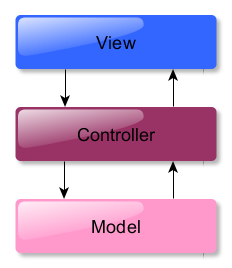
\includegraphics[scale=0.5]{figuras/modelo_mvc.PNG}
\caption{Padrão MVC - Arquitetura baseada em camadas.}
\label{modelo_mvc}
\end{figure}

A figura acima exibe o padrão arquitetural MVC - \textit{Model View Controller} -, que é uma implementação do estilo arquitetural baseado em camadas. No MVC, a camada de modelo (\textit{Model}) interage apenas com a camada de controle (\textit{Controller}). Esta, por sua vez, é responsável por promover a interação entre as camadas \textit{View} e \textit{Model}.

\subsubsection{Arquitetura Orientada a Serviços}

Este é um estilo que promove a interoperabilidade de um dado sistema, permitindo troca de dados e interação entre diversas aplicações independentemente das plataformas em que são executadas ou tecnologias utilizadas para a sua construção \cite{oqueesoa_2010}

Na arquitetura orientada a serviços, as funcionalidades ou módulos de um sistema são definidos como um serviço. Os serviços disponibilizados são expostos através do estabelecimento de contratos e interfaces de acesso e requisitados por meio do envio e recebimento de mensagens pelas aplicações \cite{oqueesoa_2010}.

\subsubsection{Arquitetura Cliente-Servidor}
O estilo arquitetural cliente-servidor é utilizado como um modelo para a implementação de sistemas distribuídos. Neste estilo, os clientes são responsáveis por realizar requisições a um conjunto de servidores que disponibilizam serviços. Geralmente, os clientes se comunicam de maneira direta com os servidores e possuem conhecimento apenas dos servidores disponíveis, desconhecendo os outros clientes existentes. Um exemplo de implementação deste estilo é a rede de uma organização onde os usuários (clientes) têm conhecimento acerca de impressoras (servidores) disponíveis. Ao acionar o serviço de impressão, o cliente estebelece uma comunicação direta com a impressora \cite{sommerville2008engenharia}.

\subsubsection{Arquitetura Baseada em Eventos}
A arquitetura baseada em eventos é um estilo arquitetural onde ocorrências importantes no sistema são identificados pelo software ou hardware que o compõe. É composta por elementos que criam um evento, que apenas sabem que um evento ocorreu e o anuncia aos demais elementos do sistema, e por aqueles que consomem os eventos anunciados. Os elementos consumidores necessitam dos eventos para realizar o processamento de uma determinada operação ou mudança de estado \cite{rouse}.

\section{SOA - Arquitetura Orientada a Serviços}

Sendo tratado como um conceito evolucionário, a orientação a serviços é uma abordagem que foi criada para a construção de sistemas de software distribuídos, a fim de promover a integração com baixo acoplamento entre aplicações e facilitar a manutenção corretiva, adaptativa ou evolutiva das mesmas \cite{linthicum_soainrealworld_2007}. Em outras palavras, a arquitetura orientada a serviços, também conhecida como SOA - do acrônimo em inglês \textit{Service-Oriented Architecture} - é "um paradigma para a construção e manutenção de processos de negócio que conecta sistemas distribuídos" \cite{josuttis_soa_2007}.

Este modelo arquitetural é utilizado para o desenho, construção, implantação e gerenciamento de sistemas de software, onde as funcionalidades deste sistema são providos por serviços que possuem interfaces de acesso bem definidas \cite{lewis_getting_2010}. Desta forma, podemos afirmar que SOA não é um tipo de tecnologia, ferramenta ou processo a serem utilizados para a construção de software, mas uma abordagem utilizada para a definição e construção da arquitetura de determinadas aplicações \cite{oliveira_interoperabilidade}.

De acordo com Josuttis \cite{josuttis_soa_2007}, SOA é um recurso a ser utilizado para construir uma arquitetura de software concreta e tem como objetivo melhorar a flexibilidade de um sistema de software, baseando-se em três conceitos técnicos principais: serviços, interoperabilidade promovida por um barramento de serviços e baixo acoplamento. SOA é uma abordagem adequada para a implementação de sistemas distribuídos em que sistemas heterogêneos são aceitos, ou seja, aplicações desenvolvidas em plataformas diferentes e em linguagens de programação distintas são capazes de interagirem formando um sistema único \cite{josuttis_soa_2007}.

A indústria de software frequentemente implementa o modelo SOA utilizando Web Services que são, de acordo com a W3C \cite{haas_web_2004}, sistemas de software construídos para dar suporte à interação ponto-a-ponto de maneira interoperável através da rede. Contudo, a orientação a serviços é algo independente de tecnologias e padrões, justificando sua implementação quando sistemas legados devem ser incorporados à arquitetura de um sistema de software \cite{linthicum_soainrealworld_2007}. A implementação deste modelo pode combinar diversas tecnologias, APIs, diferentes composições de infra-estrutura, constituindo sempre uma arquitetura única \cite{erl_orientacaoaservico_2009}.

Como qualquer modelo, SOA apresenta benefícios para a construção de software e características que podem ser ditas como desvantajosas quando este modelo é utilizado. A integração com  outros serviços, aplicativos e sistemas legados, além de prover um investimento de retorno elevado, a reutilização, flexibilidade, intereoperabilidade e governança de um serviço caracterizam algumas das vantagens relacionado ao uso este modelo \cite{oqueesoa_2010} \cite{vantagens_desvantagens_soa}. As desvantagens identificadas estão relacionados a segurança de acesso, complexidade devido à quantidade de serviços (quanto mais robusta, ou seja, quanto mais serviços, mais complexa será a arquitetura construída), performance do servidor que afeta a disponibilidade do sistema de software e a testabilidade deste  \cite{oqueesoa_2010} \cite{vantagens_desvantagens_soa}.

\subsection{Conceitos Principais}
\subsubsection{Serviços}

Serviço pode ser definido como uma aplicação de software que interage com outras aplicações por meio da troca de mensagens \cite{linthicum_soainrealworld_2007}. Além disso, um serviço é uma coleção de capacidades \cite{erl_orientacaoaservico_2009}, "é um valor entregue para outro (serviço) através de uma interface bem definida e disponível e resulta em um trabalho provido de um para outro" \cite{adaptive_ltd_service_2009}.

Um serviço é uma aplicação independente e deve ser composto por duas partes principais: a interface, que permite a comunicação com os usuários do serviços e define a estrutura das mensagens a ser utilizada para a comunicação entre um serviço e seu usuário; e a implementação, que consiste do núcleo do serviço, desconhecido pelo usuário, mas a parte responsável pela execução do serviço \cite{linthicum_soainrealworld_2007} . As principais características de um serviço, de acordo com Jossutis \cite{josuttis_soa_2007} e Erl   \cite{erl_orientacaoaservico_2009}, são:

\begin{itemize}
\item Um serviço deve ser \textbf{autônomo},  capaz de controlar seu ambiente e recursos disponibilizados. Isto implica na não interferência de fatores externos à aplicação que implementa o serviço, dependendo apenas de parâmetros fornecidos pelos usuários de um dado serviço.

\item Um serviço deve estar sempre \textbf{visível e disponível} para que possa ser descoberto e utilizado por seus usuários.

\item Um serviço deve possuir uma \textbf{alta abstração}, de modo que os detalhes de implementação sejam ocutados e apenas a interface seja acessível.

\item Um serviço \textbf{não deve guardar} informações sobre o \textbf{estado} de requisições anteriores. Informações acerca do estado de um serviço deve ser mantida apenas quando necessário.

\item Um serviço deve ser construído de modo que possa ser \textbf{reutilizado} por outras aplicações.

\item Um serviço pode ser construído a partir da \textbf{composição de outros serviços}.

\item Um serviço deve ser \textbf{idempotente}, isto é, ao ser utilizado um serviço deve retornar sempre o mesmo resultado quando os recursos disponibilizados para a sua execução forem os mesmos.

\item Um serviço deve possuir um \textbf{contrato de serviço padronizado}, que expressa o objetivo e a capacidade que o serviço implementa.
\end{itemize}

Exibir a imagem tres ponto quatro do arquivo "Services Oriented Architecture from Adobe".


\subsubsection{Baixo Acoplamento}

\subsubsection{Interoperabilidade}
usar esta referencia "Interoperabilidade em SOA Desafios e Padrões"


\subsection{Modelos de integração}
A integração entre os subsistemas de software que compõen a arquitetura distribuída de um sistema construído com base no modelo arquitetural SOA pode ser estabelecida usando-se diferentes estatégias. A estratégia utilizada para promover tal integração é um aspecto que deve ser cuidadosamente analisado, pois o impacto de tal decisão é importante e irá perpertuar-se durante a existência do produto final de software construído. Desta forma, de acordo com Bianco et. al. \cite{Bianco2007} existem duas principais abordagens para a integração entre os sistemas que compõem a implementação deste modelo:

\begin{figure}[htb]
\centering
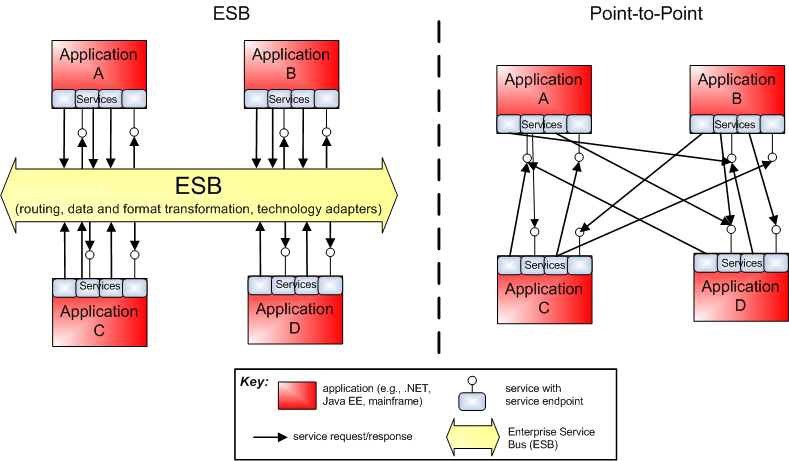
\includegraphics[scale=0.7]{figuras/modelos_integracao_soa.PNG}
\caption{Ilustração dos modelos de integração em SOA. Fonte: \cite{Bianco2007}.}
\label{modelos_integracao_soa}
\end{figure}

\begin{itemize}
\item \textbf{Direto (Ponto-a-Ponto)}: a interface de comunicação é única entre usuários e provedores de serviço; as questões relacionadas a conectividade entre os sistemas devem ser de reponsabilidade compartilhada entre tais aplicações.
\item \textbf{\textit{Hub-and-Spoke}}: a comunicação entre usuários e provedores de serviço é mediada por um terceiro software chamado ESB (\textit{Enteprise Service Bus}) ou EAI (\textit{Enterprise Application Integration}); nesta abordagem, as aplicações estebelecem uma comunicação com o ESB (ou EAI), responsável por gerenciar as mensagens enviadas pelas aplicações.
\end{itemize}

\subsection{ESB - Enterprise Service Bus}

- O que é?

- Como funciona?

- Por que usar?

- Qual a utilidade?


\subsubsection{WSO2 ESB}


\subsubsection{JBoss ESB}


\subsubsection{ErlangMS}

\section{Protocolos de Comunicação}
- O que são? Para que servem?

- Quais são os protocolos existentes? Como eles funcionam?

\subsection{SOAP}

\subsection{REST}

\section{Implementações do modelo SOA existentes}

\section{Engenharia de Software}

\subsection{Conceitos de ESW adotados}
- RUP
- Scrum